\section{Implementation}
This section will show examples from the \gls{gamble} compiler's source code which generates the object code from a \gls{gamble} program's source code.
The examples present the implementation of selected design choices made in the previous chapters.
First an example of how a \texttt{DeclarationNode} from the \acrshort{ast} is translated into C code will be provided; afterwards the implementation of using the \acrshort{gpu} using \gls{opencl} C will be presented.
The compiler starts the code generation by calling an instance of the class \texttt{CodeGenerator} and invoking the method \texttt{GenerateCodeAndWriteToFile} as can be seen on \myref{fig:CodeGeneratorVisitor}.
This method then makes the \acrshort{ast} accept a CodeGeneratorVisitor and writes its output to a file; while also exporting the object code to the \texttt{/codeout/} directory relative to the source code, along with other files needed; the \gls{opencl} kernels used in the program.
The \texttt{outputCode} is a string which starts as an empty string; every visitor then either appends or returns substrings to be appended.
These substrings add appropriate information to the \texttt{outputCode} string as the tree is traversed.

\begin{figure}
\centering
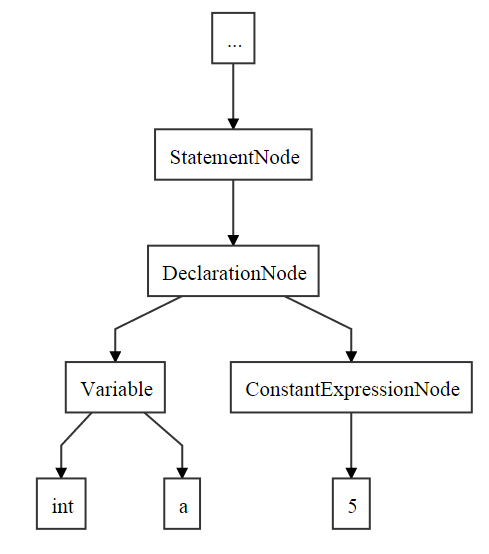
\includegraphics[width=0.5\textwidth]{figures/Trees/ASTAlone.PNG}
\caption{An \acrshort{ast} for the declaration \texttt{int a = 5;}}\label{fig:ASTAlone}
\end{figure}

\myref{fig:ASTAlone} shows a \texttt{DeclarationNode} for the expression \texttt{int a = 5;}. 
In the code generator this node will be transformed into the declaration written in C. 
The syntax for this is the same in C as it is in \gls{gamble}. 
The node has been through the previous phases, syntax and contextual analysis, where it was checked for type and scope errors, and is therefore ready to be compiled.
The code executed when the visitor accepts a \texttt{DeclarationNode} can be seen on \myref{lst:DeclarationNodeCodeGen}.
\begin{lstlisting}[float, floatplacement=H!, caption=The visit method for visiting a DeclarationNode in the code generator. ,frame=tlrb,label={lst:DeclarationNodeCodeGen}]
@Override
public String VisitDeclarationNode(DeclarationNode node) {
    String expr = "";
    String complexType = "";
    if (node.getExpression() != null){
        resultVarStack.push(node.getVariable());
        expr = visit(node.getExpression());
        resultVarStack.pop();
    }

    if (node.getVariable().isComplex()) {
        ...
    }
    if (expr.indexOf("sclManageArgsLaunchKernel
    	(hardware, software, global_size, local_size") >= 0){
        ...
    }
    
    return complexType.length() > 0 ? complexType + expr : 
    (node.getVariable().toCcode() + " = " + expr + ";");
}
\end{lstlisting}
Since the example \texttt{int a = 5;} is not of a complex data type like a matrix or vector the body of the second and third if statements are hidden.
A method is called on the node to check whether the expression that assigned the declared variable exists. 
Syntactically a matrix or vector may appear to be uninitialised but this actually creates a vector or matrix filled with zeros.
In \myref{lst:DeclarationNodeCodeGen} the expression is not null so it enters the body of the \texttt{if} statement on line 5.
The result variable, which stores the result of the expression, is pushed to a stack before visiting the expression.
In the method \texttt{VisitExpresssionNode} the top of the stack, which the result was pushed to, is checked to see if the result is a complex datatype or not; in the example the result is not of a complex data type and the expression is then evaluated by visiting the nodes of the expression.
The result of the call to \texttt{VisitExpressionNode} is saved to a string \texttt{expr}.
Another if statement checks if the declaration needs a kernel and if the expression needs to be computed on the \acrshort{gpu}.
When the call to \texttt{VisitDeclarationNode} returns; it is checked whether the length of the string \texttt{complexType} has been increased.
In the example \texttt{int a = 5;} it has not and therefore the string of the datatype and ID are concatenated with the assignment symbol, the substring \texttt{expr} and a semi-colon, before finally being returned.
